\section{Logical representation: Propositional formulas through hard activation}\label{sec:log_rep}

A tensor-based representation of propositional logic is developed by encoding boolean variables into vectors, defining formulas as boolean tensors, and showing how logical connectives and normal forms can be expressed as tensor contractions.

Here propositional logic is based on propositional formulas. Define
\begin{itemize}
    \item a \emph{propositional formula} as a boolean-valued tensor 
    \begin{align*}
        \formulaat{\shortcatvariables} \defcols \atomstates \rightarrow \ozset \subset \rr \, ,
    \end{align*}
    \item a \emph{model} of a propositional formula as a state $\shortcatindices \in \atomstates$, which fulfills 
        $% \begin{align*}
        \formulaat{\indexedshortcatvariables}=1 \, ,
    $% \end{align*}
    where we associate $\text{True}\leftrightarrow 1$ and $\text{False}\leftrightarrow 0$,
    \item and the propositional formula to be \emph{satisfiable}, if there is a model.
\end{itemize}

\begin{example}\label{ex:propform}
    The propositional formula defined for $d=3$ and $x_{[3]} = (x_1,x_2,x_3)\in \atomstates = \{0,1\}\times \{0,1\} \times \{0,1\}$ by
    \begin{align*}
        \formulaat{\shortcatvariables = x_{[3]}} = x_1 \wedge (x_2 \vee x_3)
    \end{align*}
    is satisfiable, since $\formulaat{\shortcatvariables = (1,1,1)} = 1$, $\formulaat{\shortcatvariables = (1,0,1)} = 1$, and $\formulaat{\shortcatvariables = (1,1,0)} = 1$ and therefore $x=(1,1,1)$, $x=(1,0,1)$, and $x=(1,1,0)$ are models of $\formulaat{\shortcatvariables}$.
\end{example}

Representing booleans by elements in $\{0,1\}$ leads to the problem, that negation is an affine transformation and can not be represented by multilinear tensors~\cite[Section 4.1.1]{goessmann2025}. Therefore, instead of using this \emph{coordinate calculus} an approach based on \emph{basis calculus} is employed, which is explained in this section.

This representation of propositional formulas with respect to basis encoding also leads to \ComputationActivationNetworks{}, which were also used to describe probability distributions in the last section. In this way the soft and hard logic can be combined in one framework.

\subsection{Propositional Semantics by Boolean Tensors}

To be able to express different kinds of connectives and finally any propositional formula by multi-linear tensors, booleans are encoded by one-hot encodings %vectors as
% \begin{align*}
%     \text{True}\mapsto 
%     1 \mapsto \begin{pmatrix}
%         0\\1
%     \end{pmatrix}\eqqcolon \tbasisat{Y},\\
%     \text{False}\mapsto 
%     0 \mapsto \begin{pmatrix}
%         1\\0
%     \end{pmatrix}\eqqcolon \fbasisat{Y}.
% \end{align*}
% This is the one-hot encoding of boolean states 
as defined in Definition~\ref{def:onehotenc}. 

% \begin{definition}

%     \label{def:formulas}
%     A \emph{propositional formula} $\formulaat{\shortcatvariables}$ depending on $\atomorder$ atoms $\catvariableof{\atomenumerator}$ is a boolean-valued tensor
%     \begin{align*}
%         \formulaat{\shortcatvariables} \defcols \atomstates \rightarrow \ozset \subset \rr \, .
%     \end{align*}
%     We call a state $\shortcatindices \in \atomstates$ a \emph{model} of a propositional formula $\formula$, if
%     \begin{align*}
%         \formulaat{\indexedshortcatvariables}=1 \, .
%     \end{align*}
%     If there is a model to a propositional formula, we say the formula is \emph{satisfiable}.
% \end{definition}

There are different ways to represent propositional formulas based on tensor decompositions and basis encoding representation tensors.

\paragraph{CP decomposition}
Since the tensor $\formulaat{\shortcatvariables}$ is equal to one at index $x_{[d]}$ if and only if $x_{[d]}$ is a model of $\formula$, i.e. fulfills the formula, A propositional formula can be written as the sum over the one-hot encodings of its models.
\begin{center}
    \begin{tikzpicture}[scale=0.35, thick] % , baseline = -3.5pt

%\draw[->-] (2,-1)--(2,1) node[midway,right] {\tiny $\catvariableof{\exformula}$};
\draw (-1,-1) rectangle (5,-3);
\node[anchor=center] (text) at (2,-2) {\small ${\exformula}$};
\draw[] (0,-3)--(0,-5) node[midway,left] {\tiny $\randomxof{0}$}; 
\draw[] (1.5,-3)--(1.5,-5) node[midway,left] {\tiny $\randomxof{1}$}; 
\node[anchor=center] (text) at (3,-4) {$\cdots$};
\draw[] (4,-3)--(4,-5) node[midway,right] {\tiny $\randomxof{\atomorder\shortminus1}$}; 


\node[anchor=center] (text) at (7,-2) {${=}$};

\node[anchor=center] (text) at (12,-2.5) {${\sum\limits_{\atomindices\in\atomstates}}$};
\node[anchor=center] (text) at (12,-4) {\tiny $\exformula(\atomindices)=1$};

\begin{scope}[shift={(19.5,1)}]

%\draw (-2,1) rectangle (4,-1);
%\node[anchor=center] (text) at (1,0) {\small $\onehotmapof{\exformula(\atomindices)}$};
%\draw[->-] (1,1)--(1,3) node[midway,right] {\tiny $\catvariableof{\exformula}$};

\draw (-3,-2) rectangle (-1,-4);
\node[anchor=center] (text) at (-2,-3) {\small $\onehotmapof{\atomlegindexof{0}}$};
\draw[->-] (-2,-4)--(-2,-6) node[midway,right] {\tiny $\catvariableof{0}$};

\node[anchor=center] (text) at (1,-3) {\small $\cdots$};

\draw (3,-2) rectangle (5,-4);
\node[anchor=center] (text) at (4,-3) {\small $\onehotmapof{\atomlegindexof{\atomorder\shortminus1}}$};
\draw[->-] (4,-4)--(4,-6) node[midway,right] {\tiny $\catvariableof{\atomorder\shortminus1}$};

\end{scope}

\end{tikzpicture}
\end{center}
This decomposition corresponds to the CP decomposition of a tensor.
\begin{example}
    For the formula described in Example~\ref{ex:propform}, we have
    \begin{align*}
        \formulaat{X_{[3]}} &= \left(\tbasisat{X_1} \otimes \tbasisat{X_2} \otimes \tbasisat{X_3}\right) + (\tbasisat{X_1} \otimes \fbasisat{X_2} \otimes \tbasisat{X_3}) + (\tbasisat{X_1} \otimes \tbasisat{X_2} \otimes \fbasisat{X_3}),
    \end{align*}
    where $\tbasisat{Y} = (0,1)^T$ and $\fbasisat{Y} = (1,0)^T$. Then for the model $x_{[3]} = (1,0,1)$ it holds
    \begin{align*}
        \formulaat{X_{[3]}=x_{[3]}} = &\left(\tbasisat{X_1=1} \otimes \tbasisat{X_2=0} \otimes \tbasisat{X_3=1}\right) + (\tbasisat{X_1=1} \otimes \fbasisat{X_2=0} \otimes \tbasisat{X_3=1}) \\
        &+ (\tbasisat{X_1=1} \otimes \tbasisat{X_2=0} \otimes \fbasisat{X_3=1})\\
        = & 1\cdot 0 \cdot 1 + 1\cdot 1 \cdot 1 + 1 \cdot 0 \cdot 0 = 1.
    \end{align*}
\end{example}

\paragraph{Basis encoding}
Propositional formulas $\formula$ can be expressed in terms of a tensor describing the mapping and its negation by
\begin{align}\label{eq:basisencboolean}
    \bencodingofat{\formula}{\formulavar = y,\shortcatvariables = x_{[d]}} = \begin{cases}
        1, & \formulaat{\shortcatvariables = x_{[d]}} = y\\
        0, & \text{else}
    \end{cases}.
\end{align}
This basis encoding $\bencodingofat{\formula}{\formulavar,\shortcatvariables} \in \{0,1\}^{2\times 2^d}$ then has the form
\begin{align}\label{eq:basisencnegsum}
    \bencodingofat{\formula}{\formulavar,\shortcatvariables} = \formulaat{\shortcatvariables} \otimes \tbasisat{\formulavar} + \lnot\formulaat{\shortcatvariables} \otimes \fbasisat{\formulavar}.
\end{align}
Then the propositional formula and its negation can be represented by that tensor by
\begin{align*}
    \formulaat{\shortcatvariables}
    = \contractionof{\bencodingofat{\formula}{\formulavar,\shortcatvariables},\tbasisat{\formulavar}}{\shortcatvariables}
\end{align*}
and
\begin{align*}
    \lnot\formulaat{\shortcatvariables}
    = \contractionof{\bencodingofat{\formula}{\formulavar,\shortcatvariables},\fbasisat{\formulavar}}{\shortcatvariables} \, .
\end{align*}
% which are \ComputationActivationNetworks{} to the statistic $\{\formula\}$ and the hard activation tensor $\tbasisat{\formulavar}$, respectively $\fbasisat{\formulavar}$.


As in \cite[Section 4.2.2]{goessmann2025}, in graphical notation the basis encoding has the following form.
\begin{center}
    \input{../tikz_pics/logic_representation/formula_bencoding.tex}
\end{center}

\begin{example}
     For the formula $\formulaat{X_{[1]} = x_1} = \lnot x_1$, i.e. $\formulaat{X_{[1]}} = (1, 0)^T$, we have with \eqref{eq:basisencboolean}
     \begin{center}
     \begin{tikzpicture}
         \node at (0,0) {$
         \bencodingofat{\formula}{\formulavar,X_{[1]}} = \begin{pmatrix}
             0 &1\\
             1 & 0
         \end{pmatrix}$};
         \draw[<-] (2,0.2)--(2.5,0.2);
         \node at (3.1,0.2) {$\formulavar=0$};
         \draw[<-] (2,-0.2)--(2.5,-0.2);
         \node at (3.1,-0.2) {$\formulavar=1$};
         \draw[<-] (1,-0.5)--(1,-1);
         \node at (0.5,-1.2) {$X_1=0$};
         \draw[<-] (1.4,-0.5)--(1.4,-1);
         \node at (1.9,-1.2) {$X_1=1$};
     \end{tikzpicture}
     \end{center}
     with~\eqref{eq:basisencnegsum} we have
     \begin{align*}
         \bencodingofat{\formula}{\formulavar,X_{[1]}} = \begin{pmatrix}1\\0\end{pmatrix} \otimes \begin{pmatrix}0\\1\end{pmatrix} + \begin{pmatrix}0\\1\end{pmatrix} \otimes \begin{pmatrix}1\\0\end{pmatrix}
         = \begin{pmatrix}0 &1\\0 &0\end{pmatrix} + \begin{pmatrix}0 & 0\\1 &0\end{pmatrix}
         = \begin{pmatrix}
                 0 &1\\
                 1 & 0
             \end{pmatrix}
     \end{align*} 
    and in graphical notation we get
    \begin{center}
     \begin{tikzpicture}[scale=0.35, thick] % , baseline = -3.5pt
    
        \draw[->-] (1.75,-1)--(1.75,1) node[midway,right] {\colorlabelsize $\formulavar$};
        \draw (1,-1) rectangle (3,-3);
        \node[anchor=center] (text) at (2,-2) {\corelabelsize $\bencodingof{\exformula}$};
        \draw[-<-] (1.75,-3)--(1.75,-5) node[midway,left] {\colorlabelsize $\catvariableof{0}$};

        \node[anchor=center] (text) at (5.5,-2) {${=}$};
    \begin{scope}
        [shift={(10,-0.5)}]

        \draw (-2,1) rectangle (4,-1);
        \node[anchor=center] (text) at (1,0) {\corelabelsize $\onehotmapof{1}$};
        \draw[->-] (1,1)--(1,3) node[midway,right] {\colorlabelsize $\formulavar$};

        \draw (0,-2) rectangle (2,-4);
        \node[anchor=center] (text) at (1,-3) {\corelabelsize $\onehotmapof{0}$};
        \draw[->-] (1,-4)--(1,-6) node[midway,right] {\colorlabelsize $\catvariableof{0}$};

    \end{scope}
    \node[anchor=center] (text) at (16,-2) {${+}$};
    \begin{scope}
        [shift={(21,-0.5)}]

        \draw (-2,1) rectangle (4,-1);
        \node[anchor=center] (text) at (1,0) {\corelabelsize $\onehotmapof{0}$};
        \draw[->-] (1,1)--(1,3) node[midway,right] {\colorlabelsize $\formulavar$};

        \draw (0,-2) rectangle (2,-4);
        \node[anchor=center] (text) at (1,-3) {\corelabelsize $\onehotmapof{1}$};
        \draw[->-] (1,-4)--(1,-6) node[midway,right] {\colorlabelsize $\catvariableof{0}$};

    \end{scope}
    
    \end{tikzpicture}
    \end{center}
\end{example}

\paragraph{Tensor network decomposition}
If the propositional formula allows for a decomposition into smaller propositional formulas, the representation can be reduced by employing a tensor network structure as described in the next subsection.

\paragraph{Model counts} At each index the propositional formula either carry a $1$ or $0$ encoding if the indexed value is true or false. This implies, that contracting the tensor with trivial $1$-tensors applied to each open leg leaving only one leg open results in a vector counting the number of models of the formula for each possible index of the open leg. Furthermore, contracting the whole tensor yields the number of models of the given formula. This is consistent with a probabalistic interpretation disscussed in later.

\subsection{Propositional Syntax leading to Tensor-Network Decompositions}
\begin{definition}
    Define an $r$-ary connective as a function $\circ: \times_{\ell\in[r]} [2] \to [2]$.
\end{definition}
\begin{example}\label{ex:sat_network}
    As in~\cite[Example  4.9]{goessmann2025} the following connectives are of interest.
\begin{itemize}
        \item negation $\notucon: [2]\rightarrow [2]$ by the vector
        \begin{align*}
            \notucon[\exformulavar] = \begin{bmatrix}
                                          0 \\
                                          1
            \end{bmatrix}
        \end{align*}
        \item conjunctions $\land:  [2]\times[2] \rightarrow[2]$
        \begin{align*}
            \land[\exformulavar,\secexformulavar]
            = \begin{bmatrix}
                  0 & 0 \\
                  0 & 1
            \end{bmatrix}
        \end{align*}
        \item disjunctions $\lor : [2]\times[2] \rightarrow[2]$
        \begin{align*}
            \lor[\exformulavar,\secexformulavar]
            = \begin{bmatrix}
                  0 & 1 \\
                  1 & 1
            \end{bmatrix}
        \end{align*}
        \item exact disjunction $\oplus:  [2]\times[2] \rightarrow[2]$
        \begin{align*}
            \oplus[\exformulavar,\secexformulavar]
            = \begin{bmatrix}
                  0 & 1 \\
                  1 & 0
            \end{bmatrix}
        \end{align*}
        \item implications $\impbincon:  [2]\times[2] \rightarrow[2]$
        \begin{align*}
            \impbincon[\exformulavar,\secexformulavar]
            = \begin{bmatrix}
                  1 & 1 \\
                  0 & 1
            \end{bmatrix}
        \end{align*}
        \item biimplication $\eqbincon:  [2]\times[2] \rightarrow[2]$
        \begin{align*}
            \eqbincon[\exformulavar,\secexformulavar]
            = \begin{bmatrix}
                  1 & 0 \\
                  0 & 1
            \end{bmatrix}
        \end{align*}
    \end{itemize}
    \vspace{0ex}
\end{example}
If $\formulaat{\shortcatvariables}$ is defined as the $r$-ary composition of propositional formulas $\formula_\ell, \ell\in [r]$, i.e.
\begin{align*}
    \formulaat{\shortcatvariables = x_{[d]}} = \circ\left( \formula_0\left[\shortcatvariables=x_{[d]}\right], \dots, \formula_{r-1}\left[\shortcatvariables=x_{[d]}\right]\right),
\end{align*}
then the basis encoding can be written as the contraction of the basis encoding of the $r$-ary composition and the basis encodings of the individual propositional formulas $f_\ell, \ell\in[r]$. For the composition of two propositional formulas $\formulaat{\shortcatvariables}$ and $h\left[\shortcatvariables\right]$ the composition by some binary connective is pictured below.
\begin{center}
    \input{../tikz_pics/logic_representation/unary_binarry_composition}
\end{center}
The figure can be found in~\cite[Figure 4.2 b)]{goessmann2025}, where hyperedges made up by more than two nodes represent the unaltered connection between nodes.
\begin{example}
    \alex{(see the notebook: \url{https://colab.research.google.com/drive/1p2wp61fFMu0otnfFhKoNsLiCNfWpuEsn?usp=sharing})}
    For the example described in~\cite[Figure 4.2]{goessmann2025} with the propositional formula $\formulaat{X_{[3]} = (a,b,c)}={(a \land b) \lor \lnot c}$, we can write the formula in terms of a \ComputationActivationNetwork{} with activation tensor $\tbasis$ and computation network decomposed by the basis encodings. First, it is written with one activation vector. Second, we see that it can also be interpreted with multiple features.
    \begin{center}
        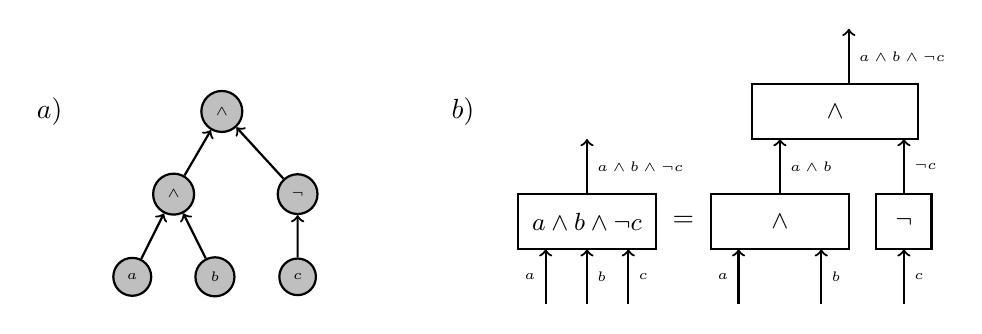
\begin{tikzpicture}[scale=0.35, yscale=-1, thick] % , baseline = -3.5pt

\begin{scope}[shift={(-15,0)}]

\node[anchor=center] (text) at (-3,-6) {${a)}$};

	\node [circle, draw, thick, fill=gray!50] (T1) at (0,0) {\tiny $\catvariableof{a}$};
	\node [circle, draw, thick, fill=gray!50] (T2) at (3,0) {\tiny $\catvariableof{b}$};
	\node [circle, draw, thick, fill=gray!50] (T3) at (6,0) {\tiny $\catvariableof{c}$};
	
	\node [circle, draw, thick, fill=gray!50] (and) at (1.5,-3) {\tiny $\land$};
	\node [circle, draw, thick, fill=gray!50] (not) at (6,-3) {\tiny $\lnot$};	
	
	\draw [->] (T1) -- (and);
	\draw [->] (T2) -- (and);
	
	\draw [->] (T3) -- (not);	
	
	\node [circle, draw, thick, fill=gray!50] (head) at (3.25,-6) {\tiny $\land$};
	
	\draw [->] (and) -- (head);
	\draw [->] (not) -- (head);			
\end{scope}

\node[anchor=center] (text) at (-3,-6) {${b)}$};

\draw[->] (0,1)--(0,-1) node[midway,left] {\tiny $\catvariableof{a}$}; 
\draw[->] (1.5,1)--(1.5,-1) node[midway,right] {\tiny $\catvariableof{b}$}; 
\draw[->] (3,1)--(3,-1) node[midway,right] {\tiny $\catvariableof{c}$}; 
\draw (-1,-1) rectangle (4, -3);
\node[anchor=center] (text) at (1.5,-2) {\small $\rencodingof{a \land b \land \lnot c}$};
\draw[->] (1.5,-3)--(1.5,-5) node[midway,right] {\tiny $\headvariableof{a \land b \land \lnot c}$}; 

\node[anchor=center] (text) at (5,-2) {${=}$};


\begin{scope}[shift={(7,0)}]

\draw[->] (0,1)--(0,-1) node[midway,left] {\tiny $\catvariableof{a}$}; 
\draw[->] (3,1)--(3,-1) node[midway,right] {\tiny $\catvariableof{b}$}; 
\draw[->] (6,1)--(6,-1) node[midway,right] {\tiny $\catvariableof{c}$}; 
	
\draw (-1,-1) rectangle (4, -3);
\node[anchor=center] (text) at (1.5,-2) {\small $\rencodingof{\land}$};

\draw[->] (1.5,-3) --(1.5,-5) node[midway,right]{\tiny $\headvariableof{a \land b}$};

\draw (5,-1) rectangle (7, -3);
\node[anchor=center] (text) at (6,-2) {\small $\rencodingof{\lnot}$};

\draw[->] (6,-3) --(6,-5) node[midway,right]{\tiny $\headvariableof{\lnot c}$};
	
\draw (0.5,-5) rectangle (6.5,-7);
\node[anchor=center] (text) at (3.5,-6) {\small $\rencodingof{\land}$};
	
\draw[->] (4,-7) -- (4,-9) node[midway,right] {\tiny $\headvariableof{a \land b \land \lnot c}$};

%\draw (3,-9) rectangle (5,-11);
%\node[anchor=center] (text) at (4,-10) {$\truevectorat{}$};

\end{scope}

\end{tikzpicture}
    \end{center}
\end{example}


\subsection{Contractions to decide entailment}
As in~\cite[Definition 5.1]{goessmann2025}, we define the entailment of two propositional formulas as follows.
\begin{definition}[Entailment of propositional formulas]
    \label{def:logicalEntailment}
    Given two propositional formulas $\kb$ and $\exformula$ we say that $\kb$ entails $\exformula$, denoted by $\kb\models\exformula$, if any model of $\kb$ is also a model of $\exformula$, that is
    \begin{align*}
        \uniquantwrtof{\shortatomindicesin}{\imppremhead{\kbat{\indexedshortcatvariables}=1}{\formulaat{\indexedshortcatvariables}=1}} \, .
    \end{align*}
    If $\kb\models\lnot\exformula$ holds, we say that $\kb$ contradicts $\exformula$.
\end{definition}
This property of interest, since $\kb$ can be chosen as a knowledge base, which can be interpreted in different ways: as the support of probability distributions, 

This is the central operation of "logical inference", i.e. deduce true statements from known statements.
One can in some cases understand this as "making the knowledge base more accessible": Adding deduced statements to a knowledge base does not change the knowledge base as a tensor, but one can interpret it in an easier way.






% \begin{example}{Sudoku rules} In case we aim to solve a Sudoku, the initial board and Sudoku rules can be written in terms of a propositional formula $\kb$. 
% To encode the Sudoku each a cell in row $\ell$ and column $k$ for $\ell,k=1,\dots,9$ can be represented by a variable r$\ell$c$k=1,\dots,9$. 
% Each Sudoku rule, e.g. that no number can be repeated in a row, can then be represented in a tensor network by a tensor connecting all variables in one row of size $9^9$.
% Technically the tensor-network contracts to the one-hot encoded unique solution, but neither is this obvious for a human seeing the initial board nor can the contraction be performed with reasonable demand. 
% Therefore, small entailment steps are done iteratively by finding and adding entailed (atomic) formulas concerning single coordinates of the solution.
% Entailments of the form
% \begin{align*}
%     \kb \models r3c5 = 7
% \end{align*}
% need to be decided, which would answer the question “Given all Sudoku rules and the initial clues, is it logically necessary that the cell in row 3, col 5 must be 7?”. Since the contraction of the whole network is infeasible, the hope is to be able to decide this by just contracting locally, e.g. checking with the initial board, if the $7$ could be somewhere else in the box in the upper box row and middle box column.
% One uses thereby the "monotonousity of entailment", i.e. when entailment holds on efficiently contractable subsets of the knowledge base then also on the full knowledge base.
% \end{example}


\begin{example}{\alex{Attempt to match the above Sudoku example with our notation of boolean variables and the entailment formalism}}
    We index the rows and the columns by tuples $(r0,r1)$ and $(co,c1)$, where $r0,r1,c0,c1\in[3]$. The first index indicates the block and the second counts the row or column inside that block.
    For each $r0,r1,c0,c1\in[3]$ and $n\in[9]$ we then define an atomic variable $\catvariableof{r0,r1,c0,c1,n}\in\{0,1\}$ indicating whether in the row $(r0,r1)$ and column $(co,c1)$ the number $n$ is written.
    The Sudoku rules then amount to the formula
    \begin{align*}
        \kb = &\left( \bigwedge_{r0,r1,c0,c1\in[3]} \left( \bigoplus_{n\in[9]} \catvariableof{r0,r1,c0,c1,n} \right) \right) \land
        \left( \bigwedge_{r0,r1\in[3], n\in[9]} \left( \bigoplus_{c0,c1\in[3]} \catvariableof{r0,r1,c0,c1,n} \right) \right) \land \\
        &\left( \bigwedge_{c0,c1\in[3], n\in[9]} \left( \bigoplus_{c0,c1\in[3]} \catvariableof{r0,r1,c0,c1,n} \right) \right) \land
        \left( \bigwedge_{r0,c0\in[3], n\in[9]} \left( \bigoplus_{r1,c1\in[3]} \catvariableof{r0,r1,c0,c1,n} \right) \right) \, ,
    \end{align*}
    where $\bigoplus$ is the $9$-ary exclusive or connective (that is $1$ if and only if exactly one of the arguments is $1$).
    The four outer brackets in $\kb$ mark the constraints, that at each position exactly one number is assigned, further that in each row each number is assigned once, and similar for the columns and the squares of the board. 
    When solving a specific Sudoku instance, one typically knows from an initial board assignment $E$ a collection of atomic variables, which hold, and needs to find further atomic variables, which are entailed.
    This means, we need to decide for each $(r_0,r_1,c_0,c_1,n)\notin E$ whether the Sudoku rules and the initial board imply that the atomic variable $\catvariableof{r0,r1,c0,c1,n}$ (i.e. assignment to the board) is true
    \begin{align*}
        \left(\kb \land \bigwedge_{(r_0,r_1,c_0,c_1,n)\in E} \catvariableof{r0,r1,c0,c1,n} \right) \models \catvariableof{r0,r1,c0,c1,n}
    \end{align*}
    or false
    \begin{align}\label{eq:sudokukb}
        \left(\kb \land \bigwedge_{(r_0,r_1,c_0,c_1,n)\in E} \catvariableof{r0,r1,c0,c1,n} \right) \models \lnot\catvariableof{r0,r1,c0,c1,n} \, .
    \end{align}
    In other words, for each assignment to the board, that fulfills the Sudoku rules and the initial board, do we write the number $n$ in row $(r0,r1)$ and column $(c0,c1)$?
    If and only if the Sudoku has a unique solution given the initial board assignment $E$, exactly one of these entailment statements holds for each $(r_0,r_1,c_0,c_1,n)\notin E$.
    Deciding which is equivalent to solving of the Sudoku.
\end{example}

In the tensor network representation, these entailments can be decided by contracting the whole representing tensor with the statement, that needs to be checked.

% \alex{Maybe we use directly a contraction based definition of entailment (Theorem 5.2 in the report):}

\begin{theorem}[{Entailment in propositional logic~\cite[Theorem 5.2]{goessmann2025}}]
    For two propositional formulas $\kb$, $\exformula$ we have
    \begin{align*}
        \kb\models\exformula \iff \contraction{\kb,\lnot\exformula}=0 \, .
    \end{align*}
\end{theorem}

Since contracting the whole tensor is often infeasible and for instance for the Sudoku example would correspond to solving the whole problem, local contractions can be considered to decide in some cases.
Here a local contraction describes the calculation of contractions along few closely connected legs in the tensor network. Now, if the local contraction of any legs leads to a zero-tensor in the network decomposition, the whole contraction amounts to zero, and the knowledge base entails $f$.

\begin{example}{Sudoku continued}
For the Sudoku example, a local contraction of the left- and right-hand-side of~\eqref{eq:sudokukb} means that only direct connections via the basic Sudoku rules and the known board are checked. If the local contraction amounts to zero, the direct Sudoku rules already imply, that $X_{r0,r1,c0,c1,n}$ must be true/is the only possible choice. In most cases the local contraction will not lead to $0$. Then no statement can be made.
\end{example}

% By~\cite[Theorem 5.2]{goessmann2025} the following statements hold:
% \begin{align*}
%     \kb \text{ entails } \exformula \text{ i.e. } \kb\models\exformula &\iff \contraction{\kb,\lnot\exformula} = 0 \text{ and }\\
%     \kb \text{ contradicts } \exformula \text{ i.e. } \kb\models\lnot\exformula &\iff \contraction{\kb,\exformula} = 0.
% \end{align*}
% Additionally, a tensor can be defined, which can encode entailment and contradiction properties simultaneously, see~\cite[Theorem 5.3]{goessmann2025}.




\subsection{Representation of Knowledge Bases}

When having multiple formulas: Represent with multiple $\tbasis$ activation cores~\cite[Theorem 14.36]{goessmann2025}. 

\begin{align*}
    \contractionof{\tbasisat{\headvariable},\bencodingofat{\land}{\headvariable,\shortcatvariables}}{\shortcatvariables}
    =
    \bigotimes_{\catenumeratorin} \tbasisat{\catvariableof{\catenumerator}}
\end{align*}

Noting that for example for $x_a=x_b=\epsilon_1=[0,1]^\intercal$
\begin{center}
    \input{../tikz_pics/logic_representation/and_decomposition}
\end{center}
while for all other vectors $x_a,x_b$, all parts of the equations amount to $0$. This yields that a knowledge base consisting of multiple formulas connected by a $\land$ has an efficient representation by decomposing the the tensor into its individual formulas.